\chapter{Laboratorio 1}
\section{Introduzione}
Il primo circuito realizzato in laboratorio è un \textit{emmitter follower}, di cui si riporta di seguito lo schematico:
\begin{figure}[h!]
	\centering
	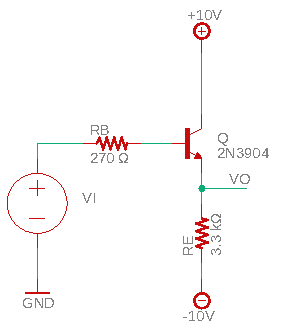
\includegraphics[width=0.4\linewidth]{./OtherFiles/Laboratorio 1/emitter follower}
	\caption{Schematico del circuito emitter follower.}
	\label{fig:emitterfollwer}
\end{figure}

\section{Punto di lavoro}
Per analizzare il circuito, si procede all'analisi del punto di lavoro, dove i generatori di tensioni e correnti alternate vengono sostituiti rispettivamente con un corto circuito o un circuito aperto (\Fig\ref{fig:emitterfollwer_puntodilavoro}).
\begin{figure}[h!]
	\centering
	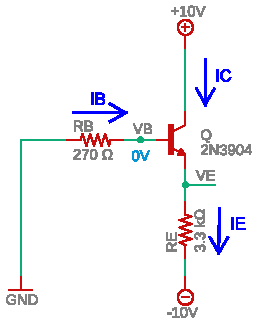
\includegraphics[width=0.4\linewidth]{./OtherFiles/Laboratorio 1/emitter follower_punto di lavoro_printout}
	\caption{Analisi del punto di lavoro del circuito emitter follower.}
	\label{fig:emitterfollwer_puntodilavoro}
\end{figure}
In particolare, il generatore di tensione (di segnale) V\textsubscript{in} viene quindi considerato come un corto circuito che collega un terminale della resistenza R\textsubscript{B} a massa. Considerando il modello ideale del transistor Q , con $\beta\overrightarrow{}\infty$ e corrente di base nulla, si ricava che la corrente che attraversa la resistenza R\textsubscript{B} è nulla. Per cui, per la legge di Ohm $V=R*I$, la caduta di potenziale sulla resistenza è nulla. Per cui il nodo V\textsubscript{B} si trova a una tensione di \SI{0}{\volt}. 

Se si esegue un bilancio di correnti delle correnti uscenti e entranti nel transistor si ottiene $I\sub{B}+I\sub{C}=I\sub{E}$. Dal momento che la corrente I\sub{B} è nulla, I\sub{C} = I\sub{E}.

Supponendo che il transistor si trovi in regione attiva diretta, $V_{BE}=V_{BO}=+\SI{0.7}{\volt}$. Quindi, $V_O=V_B-\SI{0.7}{\volt}= -\SI{0.7}{\volt}$.

Infine, la corrente di emettitore (e di conseguenza anche la corrente di collettore) si ricava dalla legge di Ohm: $I_E=I_C=\frac{\Delta V}{R_E}=\frac{V_O-(-\SI{10}{\volt})}{R_E}$. 

Come si può notare, si verifica l'ipotesi che il transistor si trova in regione attiva diretta, dal momento che $V_{CB}>0$.

Avendo ricavato la corrente di collettore stazionaria, è utile calcolare anche la transcoduttanza del transistor: $g_m=\frac{I_C^*}{\phi_T}$, con $I_C^*$ corrente di collettore stazionaria e $\phi_T\simeq\SI{26}{\milli\volt}$. Essa sarà utile nell'analisi di piccolo segnale.

Nella seguente tabella, si riportano i valori teorici delle diverse grandezze che determinano il punto di lavoro e che dovranno essere confrontate con i valori misurati sul circuito reale.

\begin{table}[h!]
	\centering
	\begin{tabular}{c|c|c|c|c|c}
		\hline
		V\sub{B} [V] & V\sub{O} [V] & I\sub{B} [A] & I\sub{E} [mA] & I\sub{C} [mA] & g\sub{m} [A/V]\\ \hline
		0 & -0.7 & 0 & 2.818 & 2.818 & 0.1084\\ \hline
	\end{tabular}
\end{table}

\section{Analisi per piccolo segnale}
Consideriamo ora l'analisi per piccolo segnale del circuito, sostituendo il transistor con il modello semplificato senza resistenza di base. Si procede quindi anche spegnere i generatori di grandezze continue ottenendo il circuito mostrato in figura \ref{fig:emitterfollwer_piccolo segnale}. Come si può notare, il transistor è sostituito da un generatore di corrente ideale controllato dalla tensione $v_{be}$ e il terminale di base rimane isolato rispetto al collettore e all'emettitore. La transcoduttanza \textit{g\sub{m}} è quella calcolata nell'analisi DC.
\begin{figure}[h!]
	\centering
	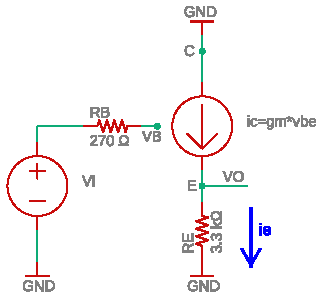
\includegraphics[width=0.4\linewidth]{./OtherFiles/Laboratorio 1/emitter follower_piccolo segnale_printout}
	\caption{Analisi di piccolo segnale del circuito emitter follower.}
	\label{fig:emitterfollwer_piccolo segnale}
\end{figure}
Si noti che la tensione v\sub{B} è pari a v\sub{i}, poiché la corrente nella resistenza R\sub{B} è nulla.
Per calcolare la funzione di trasferimento tra la tensione in ingresso (v\sub{i}) e la tensione in uscita (v\sub{o}) calcoliamo il bilancio di correnti al nodo \textbf{E}:
\begin{equation}
	\begin{split}
		i_c&=g_m * v_{be} = i_e \\ 
		v_b&=v_i \\
		i_c&=g_m*(v_B-v_E)=g_m*(v_i-v_o) \\
		i_e&=\frac{v_e-\SI{0}{\volt}}{R_E}=\frac{v_o}{R_E} \\
		\frac{v_o}{R_E}&=g_m*(v_i-v_o) \\
		\frac{v_o}{v_i}&=\frac{g_m*RE}{1+g_m*R_E}\simeq 1, \; per \; g_m*R_E\gg 1 \\
	\end{split}
\end{equation}
\todo{controllare lettere maiuscole e minuscole correnti tensioni}
Si realizza quindi un circuito in cui l'uscita insegue esattamente l'andamento della tensione in ingresso.

\section{Componenti e misure}
Il circuito è stato realizzato in laboratorio su una breadboard e il risultato è visibile in figura \ref{fig:emitterfollwer_circuito}. Inizialmente, non è stato collegato il generatore di forme d'onda \textit{v\sub{i}}, sostituendolo con un collegamento a massa. In questo modo è possibile effettuare l'analisi del punto di lavoro del circuito.
\begin{figure}[h!]
	\centering
	\includegraphics[width=0.4\linewidth]{./ImageFiles/Laboratorio 1/IMG\_20220510\_103526}
	\caption{Foto del circuito realizzato in laboratorio.}
	\label{fig:emitterfollwer_circuito}
\end{figure}

Per realizzare il circuito sono stati utilizzati i seguenti componenti: 
\begin{itemize}
	\item transistor 2N3904;
	\item una resistenza da \SI{270}{\ohm} per realizzare la resistenza R\sub{B};
	\item due resistenze rispettivamente da \SI{1.5}{\ohm} e \SI{1.8}{\ohm} connesse in parallelo per realizzare la resistenza R\sub{E}.
\end{itemize}
Inoltre, sono state utilizzate i seguenti strumenti:
\begin{itemize}
	\item alimentatore da banco con tensione positiva \SI{10}{\volt}, tensione negativa \SI{-10}{\volt} e limite in corrente di \SI{50}{\milli\ampere};
	\item oscilloscopio a due canali;
	\item generatore di forme d'onda;
	\item multimetro da banco.
\end{itemize}

Prima di utilizzare i componenti sono stati misurati, attraverso il multimetro, i valori di resistenze e delle tensioni delle giunzioni P-N tra \textit{base} e \textit{collettore} e tra \textit{base} e \textit{emettitore} del transistor, ottenendo le seguenti misure:

\begin{table}[h!]
	\centering
	\begin{tabular}{c|c|c}
		\hline
		Componente & Valore nominale & Valore misurato \\ \hline
		R\sub{B} & \SI{270}{\ohm} & \SI{278.56}{\ohm}  \\ \hline
		R\sub{E1} &\SI{1.5}{\kilo\ohm} & \SI{1.495}{\kilo\ohm} \\ \hline
		R\sub{E2} &\SI{1.8}{\kilo\ohm} & \SI{1.810}{\kilo\ohm} \\ \hline
		Vd\sub{B-E} & $\simeq$ \SI{0.7}{\volt} & \SI{0.700}{\volt} \\ \hline
		Vd\sub{B-C} & $\simeq$ \SI{0.7}{\volt} & \SI{0.679}{\volt} \\ \hline
	\end{tabular}
\end{table}
Si noti che le tensioni delle giunzioni P-N hanno valori diversi: ciò è dovuto alla tecnologia di realizzazione del transistor (tecnologia planare), nella quale le due giunzioni hanno una diversa lunghezza.

Una volta realizzato il circuito sono state poi misurate le tensioni ai nodi V\sub{B} e V\sub{O} da cui è stato possibile ricavare (tramite la legge di Ohm) le correnti di base, di emettitore. Inoltre, è stata anche calcolata la transcoduttanza. La corrente di collettore è stata ricavata come differenza tra la corrente di emettitore e corrente di base. 

Sono stati ottenuti i seguenti valori:
\begin{table}[h!]
	\centering
	\begin{tabular}{c|c|c|c|c|c}
		\hline
		V\sub{B} [mV] & V\sub{O} [V] & I\sub{B} [mA] & I\sub{E} [mA] & I\sub{C} [mA] & g\sub{m} [A/V]\\ \hline
		-3.82 & -0.655 & 0.014 & 2.819 & 2.805 & 0.1079\\ \hline
	\end{tabular}
\end{table}
I valori misurati si avvicinano ai valori calcolati nell'analisi teorica del punto stazionario (a meno di approssimazioni e errori di misura). In particolare, si noti come la corrente di base sia molto piccola (\SI{14}{\micro\ampere}) e la tensione V\sub{O} che equivale alla tensione della giunzione P-N tra base e emettitore in regione diretta.

Successivamente, si è applicato un segnale sinusoidale v\sub{i} tramite un cavo di tipo BNC collegato al generatore di forme d'onda, impostando una frequenza pari a \textit{f=}\SI{1}{\kilo\hertz} e una tensione picco-picco \textit{V\sub{pp}=}\SI{2}{\volt}. Collegando opportunamente i connettori dell'oscilloscopio, è stato possibile misurare il segnale in ingresso e in uscita al circuito e verificare che il guadagno del circuito fosse unitario.
\begin{figure}[h!]
	\centering
	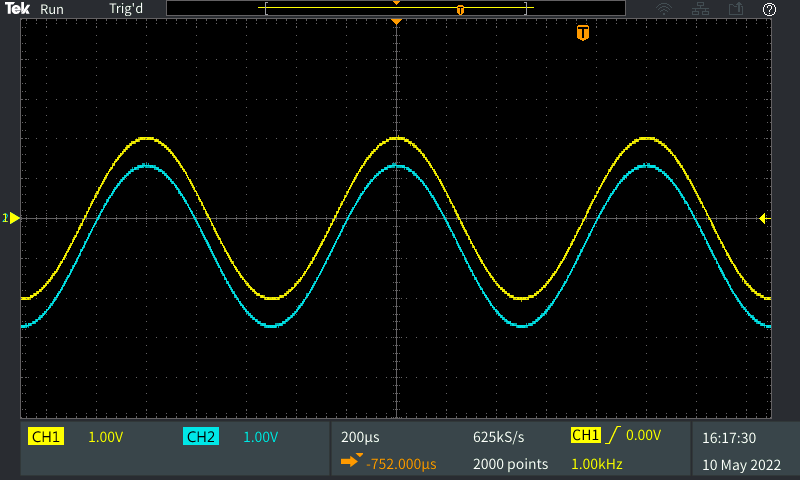
\includegraphics[width=0.7\linewidth]{./ImageFiles/Laboratorio 1/TEK00005}
	\caption{Segnale in ingresso (CH1) e in uscita (CH2) all'emitter follower misurato con l'oscilloscopio. Onda sinusoidale in ingresso con frequenza \SI{1}{\kilo\hertz} e tensione picco-picco di \SI{2}{\volt}.}
	\label{fig:emitterfollwer_oscilloscopio_1}
\end{figure}
Si noti come il segnale giallo (ingresso) e il segnale azzurro (uscita) abbiamo uguale ampiezza e fase. Per verificare che lo sfasamento sia nullo, è stata selezionata la modalità XY sull'oscilloscopio (\Fig\ref{fig:emitterfollwer_XY_1}).
\begin{figure}[h!]
	\centering
	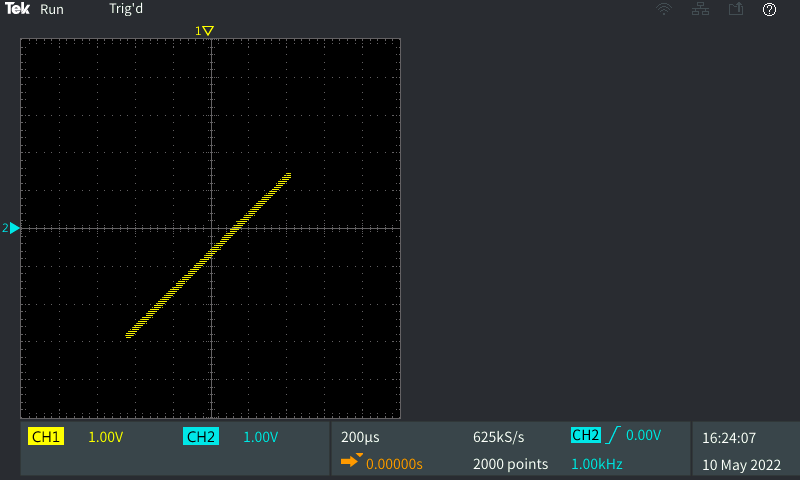
\includegraphics[width=0.7\linewidth]{./ImageFiles/Laboratorio 1/TEK00008}
	\caption{Grafico XY con onda sinusoidale in ingresso con frequenza \SI{1}{\kilo\hertz} e tensione picco-picco di \SI{2}{\volt}.}
	\label{fig:emitterfollwer_XY_1}
\end{figure}
Come si può notare, la presenza di un segmento con inclinazione di 45 gradi indica che i segnali sono in fase. Inoltre, si noti l'offset di circa \SI{0.7}{\volt}, dovuto alla giunzione base-collettore. 
Tuttavia, aumentando la frequenza dell'onda sinusoidale fino ai \SI{10}{\mega\hertz} si noti come il circuito introduce uno sfasamento. Infatti, a frequenze elevate gli effetti delle capacità parassite presenti nel transistor diventano significativi, introducendo un comportamento simile a un filtro passa-basso. Per questo motivo, il grafico XY (\Fig\ref{fig:emitterfollwer_XY_2}) non mostra più un segmento ma un ellissi, indicando la presenza di uno sfasamento. 
\begin{figure}[h!]
	\centering
	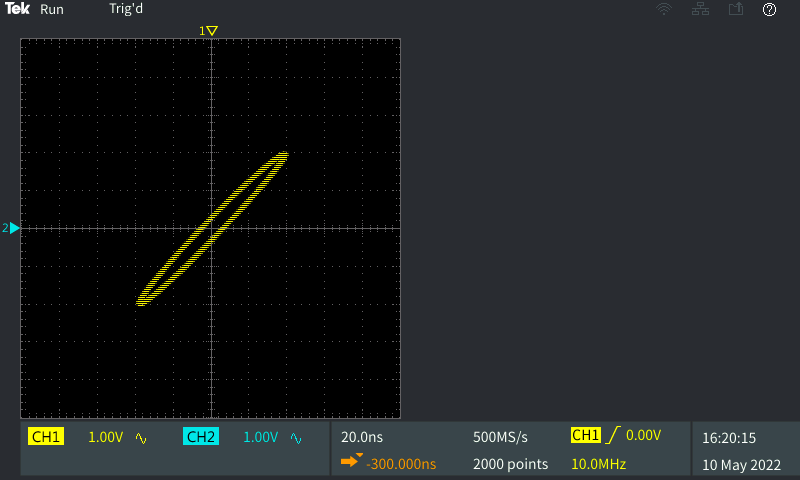
\includegraphics[width=0.7\linewidth]{./ImageFiles/Laboratorio 1/TEK00006}
	\caption{Grafico XY con onda sinusoidale in ingresso con frequenza \SI{10}{\mega\hertz} e tensione picco-picco di \SI{2}{\volt}. I segnali in ingresso sono stati accoppiati in AC.}
	\label{fig:emitterfollwer_XY_2}
\end{figure}
Lo sfasamento è visibile anche utilizzando la rappresentazione sull'asse dei tempi come mostrato in figura \ref{fig:emitterfollwer_oscilloscopio_2}.
\begin{figure}[h!]
	\centering
	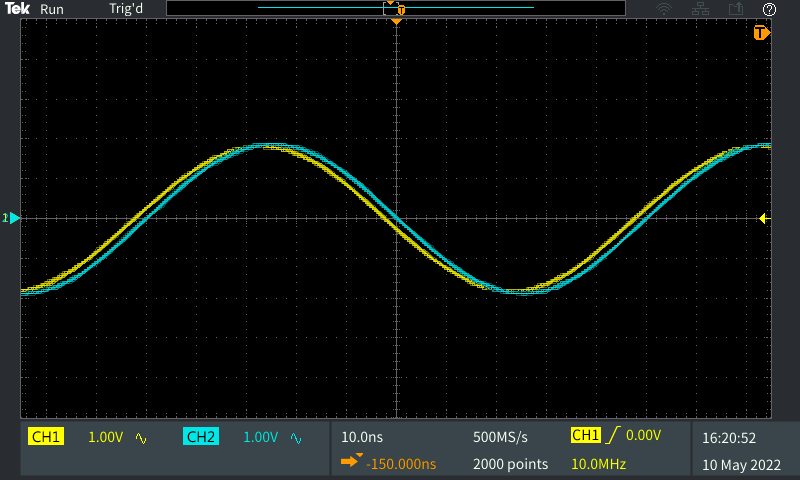
\includegraphics[width=0.7\linewidth]{./ImageFiles/Laboratorio 1/TEK00007}
	\caption{Segnale in ingresso (CH1) e in uscita (CH2) all'emitter follower misurato con l'oscilloscopio. Onda sinusoidale in ingresso con frequenza \SI{10}{\mega\hertz} e tensione picco-picco di \SI{2}{\volt}. I segnali in ingresso sono stati accoppiati in AC.}
	\label{fig:emitterfollwer_oscilloscopio_2}
\end{figure}

\todo{e il guadagno?? laboratorio dopo}